\documentclass[11pt]{article}
\usepackage[utf8]{inputenc}
\usepackage{amsmath}
\usepackage{amsfonts}
\usepackage{amssymb}
\usepackage{graphicx}
\usepackage{booktabs}
\usepackage{hyperref}
\usepackage{caption}
\usepackage{subcaption}
\usepackage{geometry}
\geometry{margin=1in}

\title{Bayesian Neural Networks: Comparative Analysis and Implementation Report}
\author{College Project}
\date{\today}

\begin{document}

\maketitle

\begin{abstract}
This report presents a comparative analysis of Bayesian Neural Network (BNN) implementations, focusing on two primary approaches: Laplace approximation and Stochastic Variational Inference (SVI) via Flipout estimators. The analysis covers applications to both sinusoidal regression tasks and poverty mapping using satellite imagery from the WILDS PovertyMap dataset. We evaluate these methods in terms of uncertainty quantification, computational efficiency, and predictive performance.
\end{abstract}

\section{Introduction}
Bayesian Neural Networks extend standard neural networks by placing prior distributions over weights and computing posterior distributions, enabling uncertainty quantification in predictions. This report examines two distinct BNN methodologies:
\begin{enumerate}
    \item Laplace approximation (post-hoc Gaussian approximation around MAP estimate)
    \item Bayesian-Torch with SVI using Flipout estimators (learned variational posterior)
\end{enumerate}

We analyze these approaches across two different domains:
\begin{itemize}
    \item Sinusoidal regression task (1D function approximation)
    \item PovertyMap satellite imagery analysis (WILDS benchmark)
\end{itemize}

\section{Methodology}

\subsection{Theoretical Background}

\subsubsection{Laplace Approximation}
The Laplace method approximates the posterior distribution around a Maximum A Posteriori (MAP) estimate with a Gaussian distribution:
\[
\mathcal{N}(w_{MAP}, H^{-1})
\]
where $H$ is the Hessian of the loss with respect to parameters. In our implementations, we use:
\begin{itemize}
    \item Full covariance approximation for the last layer
    \item Generalized Linear Model (GLM) predictive distribution
    \item Hyperparameter tuning via marginal likelihood minimization
\end{itemize}

\subsubsection{Bayesian-Torch with Flipout SVI}
This approach learns a variational posterior alongside network weights using Stochastic Variational Inference:
\begin{itemize}
    \item Flipout estimator to reduce variance in Monte Carlo sampling
    \item Evidence Lower Bound (ELBO) optimization
    \item MC sampling for predictive distribution approximation
\end{itemize}

\subsection{Evaluation Metrics}
Both methodologies are evaluated using:
\begin{itemize}
    \item \textbf{RMSE}: Root Mean Squared Error (point prediction accuracy)
    \item \textbf{NLL}: Negative Log-Likelihood (predictive distribution quality)
    \item \textbf{Calibration Error}: Uncertainty calibration quality
\end{itemize}

\section{Experimental Results}

\subsection{Sinusoidal Regression Task}

The sinusoidal regression experiment compared MAP baseline, Laplace-Torch, and Bayesian-Torch on a 1D function approximation task with known noise level $\sigma=0.3$.

Key architectural choices:
\begin{itemize}
    \item Network: Linear(1,50) → Tanh → Linear(50,1)
    \item Shared MAP-trained deterministic network as starting point
    \item Laplace: Full Hessian approximation with GLM predictive
    \item Bayesian-Torch: Flipout layers with MOPED initialization and ELBO fine-tuning
\end{itemize}

Results summary (as shown in the notebook):
\begin{table}[htbp]
\centering
\caption{Comparison of BNN methods on sinusoidal regression}
\begin{tabular}{lccc}
\toprule
\textbf{Metric} & \textbf{Laplace-Torch} & \textbf{Bayesian-Torch} & \textbf{MAP (Baseline)} \\
\midrule
Type & Post-hoc Laplace & SVI (Flipout) & Deterministic \\
Inference & Closed-form (GLM) & MC sampling & Simple Feed-Forward \\
Uncertainty & Local Gaussian approx & Learned variational & None \\
Time taken & Measured locally & Measured locally & Measured locally \\
\bottomrule
\end{tabular}
\end{table}

\subsection{PovertyMap Satellite Imagery Analysis}

The PovertyMap experiment applied BNNs to predict asset wealth index from satellite imagery using a ResNet-18 architecture.

Key aspects of this experiment:
\begin{itemize}
    \item Dataset: WILDS PovertyMap benchmark (satellite images, 224×224, 8 multi-spectral bands)
    \item Architecture: ResNet-18 adapted for 8-channel inputs
    \item Evaluation: 5-fold cross-validation across country splits (Folds A-E)
    \item Metrics: RMSE, NLL, Regression Calibration Error
\end{itemize}

Methodological differences:
\begin{enumerate}
    \item \textbf{Laplace method}: Last-layer Laplace with full covariance approximation, GLM predictive distribution (2,000 samples), hyperparameters tuned by minimizing NLL on ID validation set
    \item \textbf{Bayesian-Torch}: Variational posterior via SVI using Flipout estimators, MC sampling (50 samples for validation)
\end{enumerate}

The experiment structurally compiled theoretical capabilities, training/inference time overheads, and performance metrics across folds.

\section{BNN Libraries Overview}

A survey of popular BNN libraries reveals different approaches to Bayesian deep learning:

\begin{table}[htbp]
\centering
\caption{Comparison of BNN libraries}
\begin{tabular}{lp{4cm}p{3cm}p{2cm}}
\toprule
\textbf{Library} & \textbf{Based on} & \textbf{Implementation} & \textbf{Notes} \\
\midrule
BI & NumPyro/TFP (JAX framework) & & Leverages PPLs for HPC and AD \\
PyMC & PyTensor & Variational Inference / MCMC sampling & MCMC and ADVI \\
Bayes-Torch & PyTorch & stochastic VI (BBB) & reparam MC estimators and flipout \\
Laplace-Torch & PyTorch & Laplace approximation & \\
TyXe & PyTorch & VI / MCMC & \\
BLiTZ & PyTorch & VI BBB & \\
\bottomrule
\end{tabular}
\end{table}

\section{Visualizations}

Figures generated during experimentation illustrate key concepts and results:

\begin{figure}[htbp]
\centering
\begin{subfigure}[b]{0.45\textwidth}
    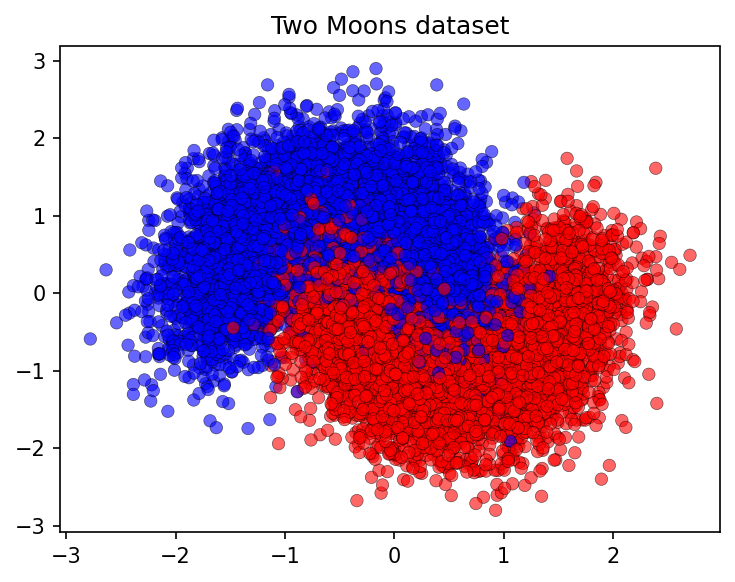
\includegraphics[width=\textwidth]{./laplace_torch/figures/01_raw_dataset.png}
    \caption{Raw sinusoidal dataset}
\end{subfigure}
\hfill
\begin{subfigure}[b]{0.45\textwidth}
    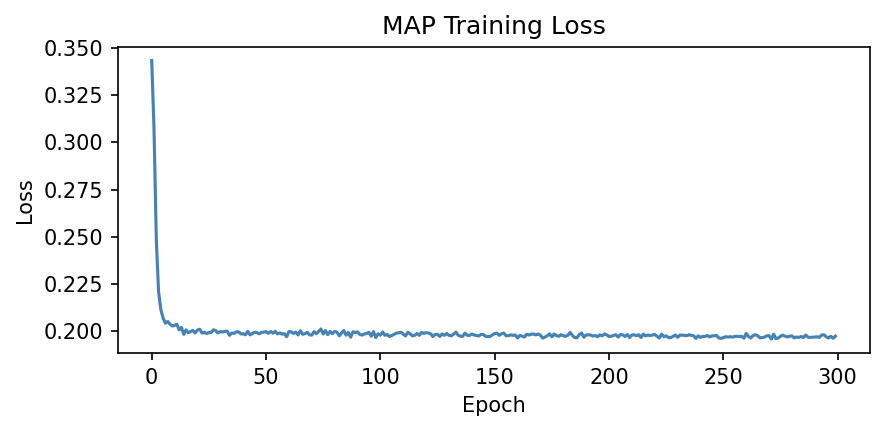
\includegraphics[width=\textwidth]{./laplace_torch/figures/02_map_training_loss.png}
    \caption{MAP training loss}
\end{subfigure}
\caption{Initial data visualization and MAP training progress}
\end{figure}

\begin{figure}[htbp]
\centering
\begin{subfigure}[b]{0.45\textwidth}
    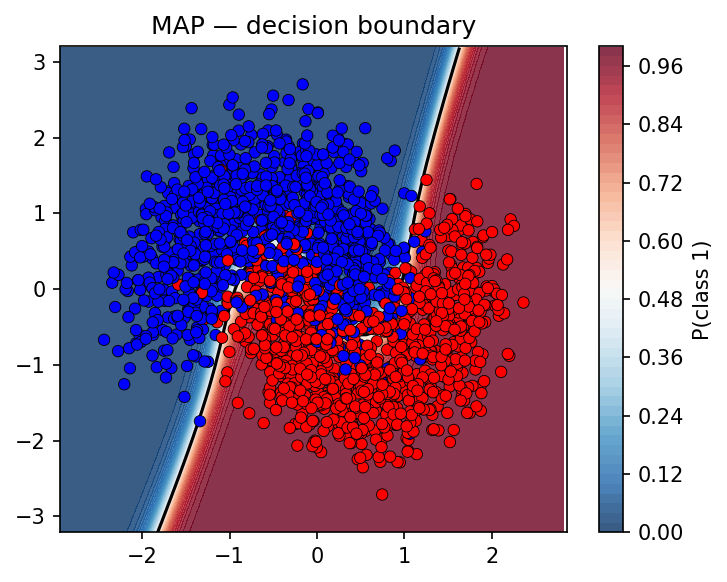
\includegraphics[width=\textwidth]{./laplace_torch/figures/03_map_boundary.png}
    \caption{MAP decision boundary}
\end{subfigure}
\hfill
\begin{subfigure}[b]{0.45\textwidth}
    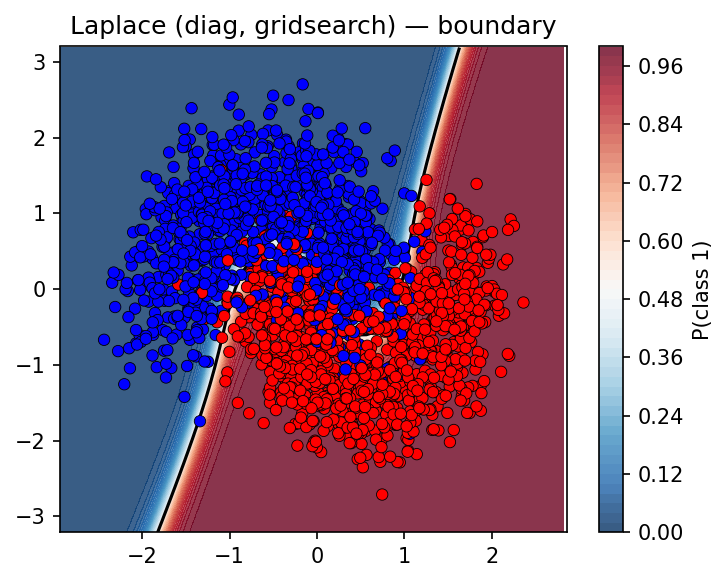
\includegraphics[width=\textwidth]{./laplace_torch/figures/04_laplace_diag_grid_boundary.png}
    \caption{Laplace diagonal grid boundary}
\end{subfigure}
\caption{Comparison of MAP and Laplace approximation boundaries}
\end{figure}

\begin{figure}[htbp]
\centering
\begin{subfigure}[b]{0.45\textwidth}
    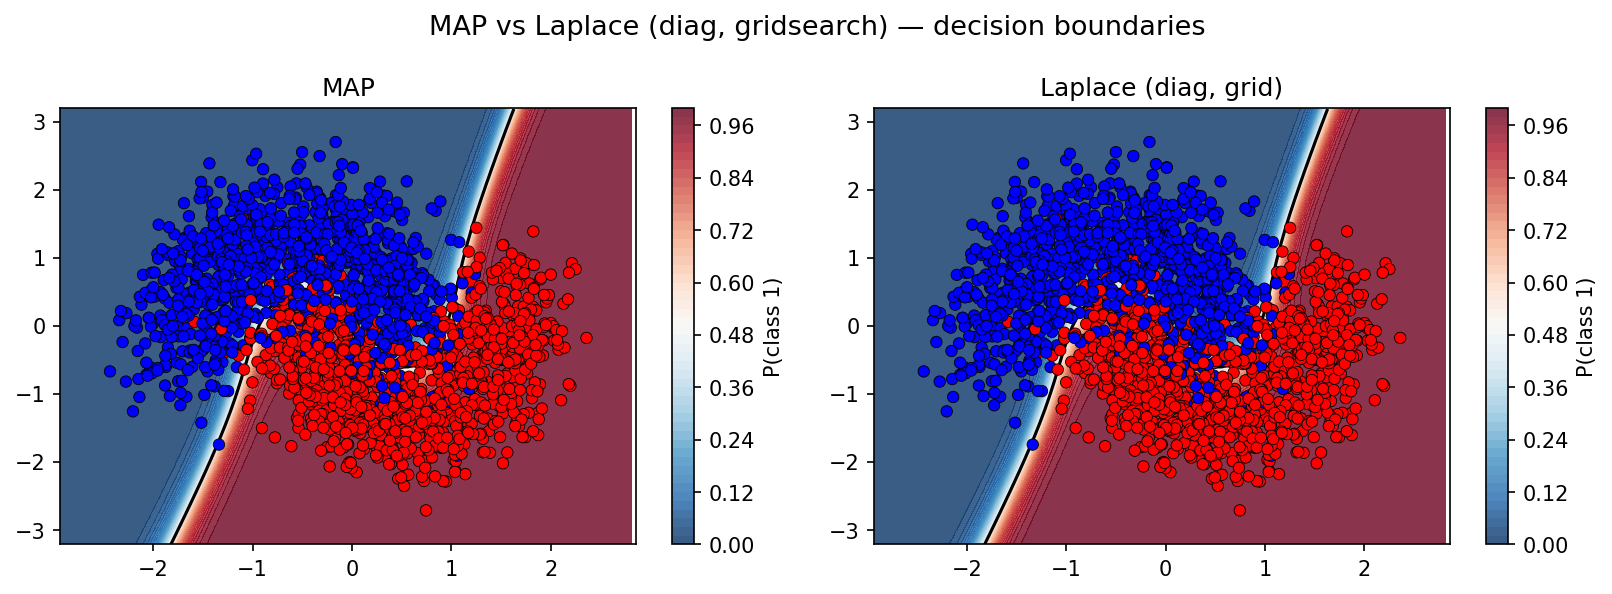
\includegraphics[width=\textwidth]{./laplace_torch/figures/05_map_vs_laplace_boundary.png}
    \caption{MAP vs Laplace boundary}
\end{subfigure}
\hfill
\begin{subfigure}[b]{0.45\textwidth}
    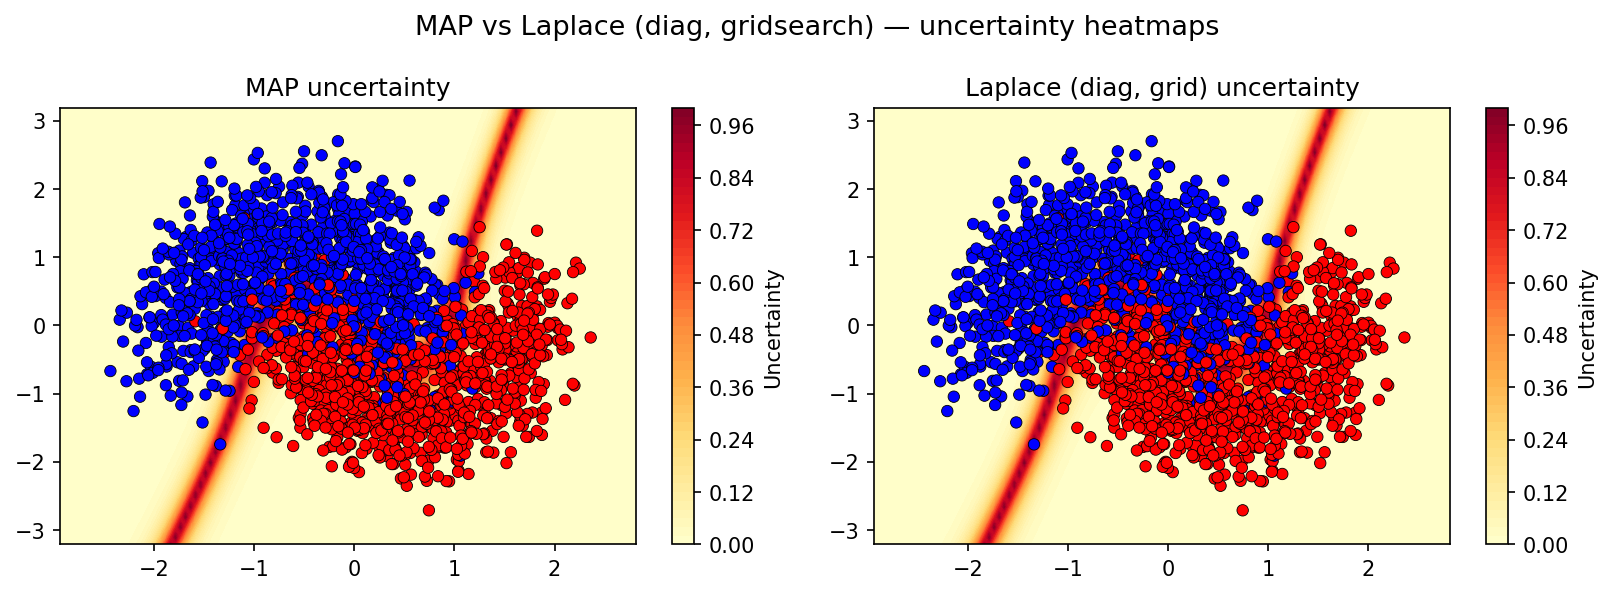
\includegraphics[width=\textwidth]{./laplace_torch/figures/06_map_vs_laplace_uncertainty.png}
    \caption{MAP vs Laplace uncertainty}
\end{subfigure}
\caption{Boundary and uncertainty comparisons between MAP and Laplace methods}
\end{figure}

\begin{figure}[htbp]
\centering
\begin{subfigure}[b]{0.45\textwidth}
    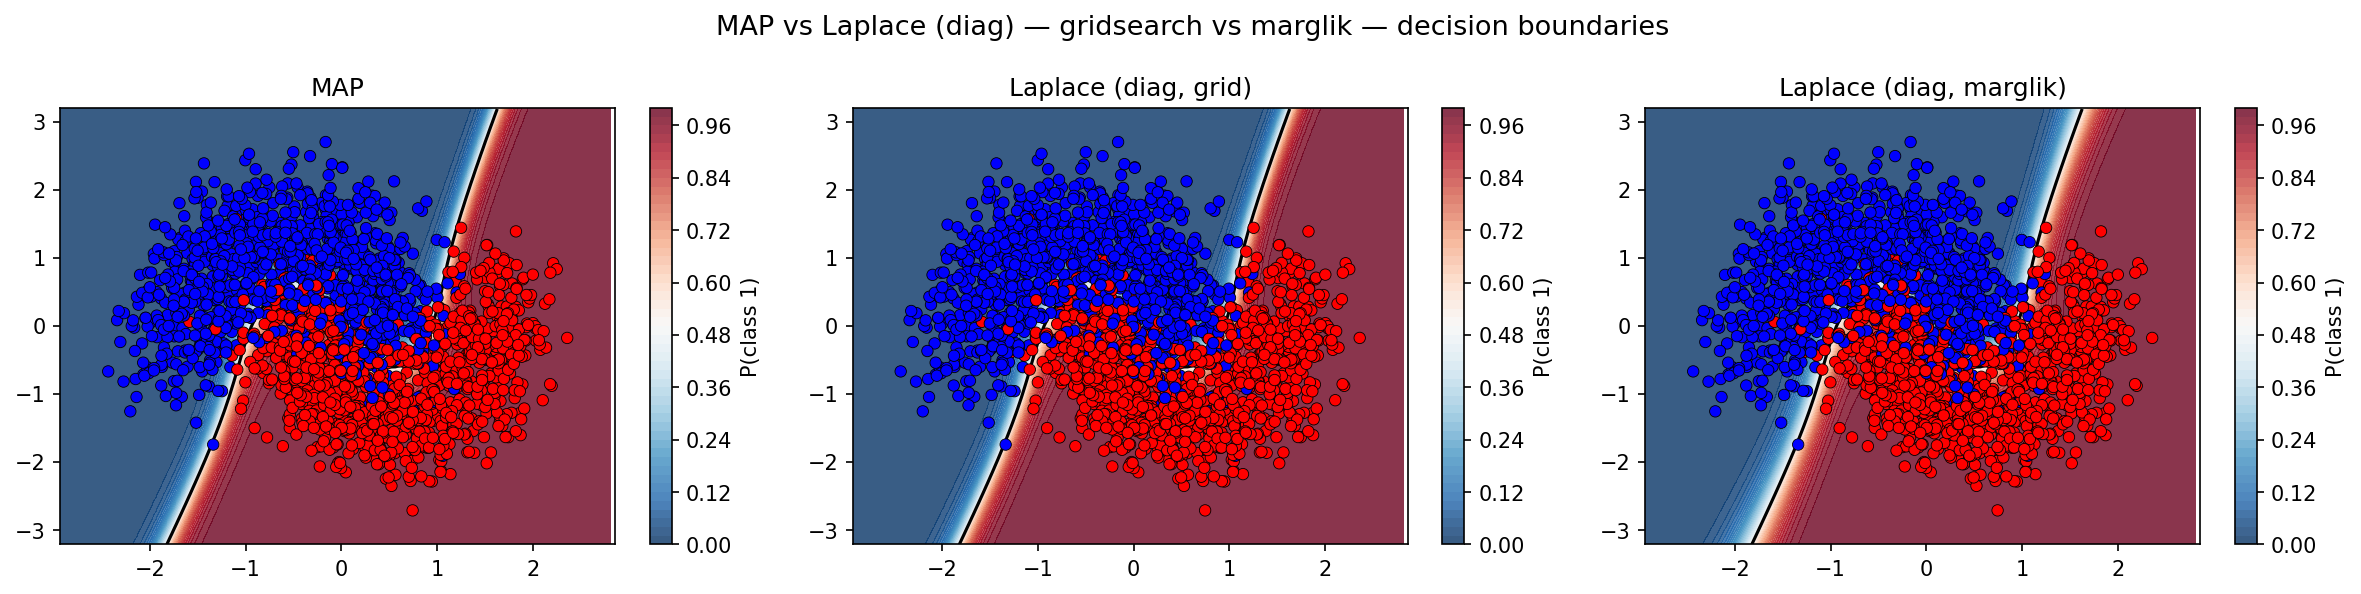
\includegraphics[width=\textwidth]{./laplace_torch/figures/07_three_way_boundary.png}
    \caption{Three-way boundary comparison}
\end{subfigure}
\hfill
\begin{subfigure}[b]{0.45\textwidth}
    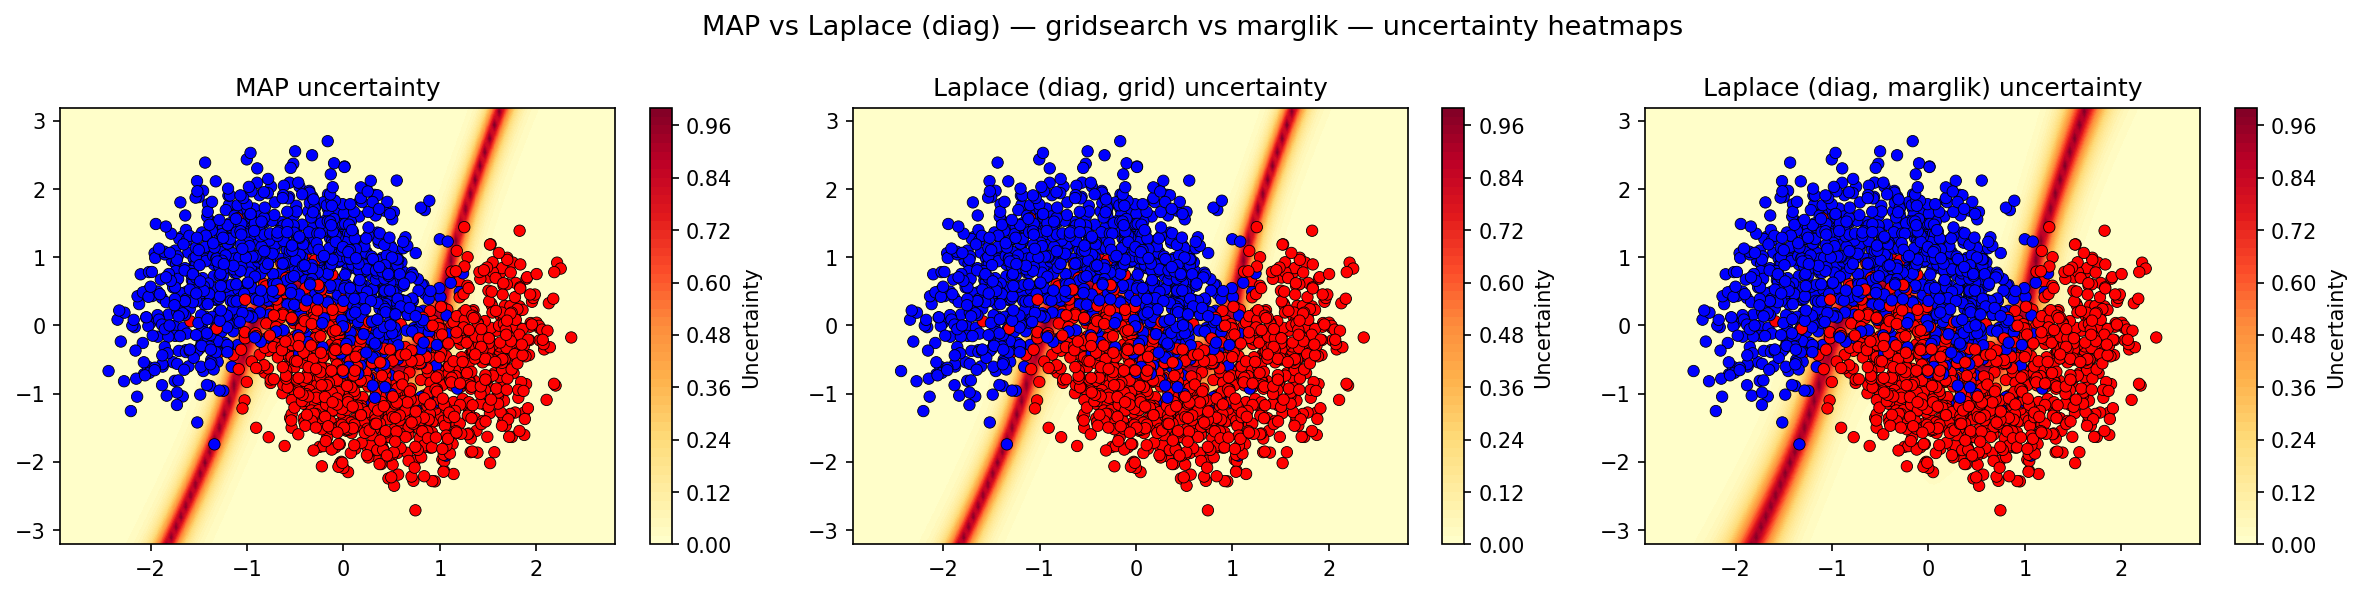
\includegraphics[width=\textwidth]{./laplace_torch/figures/08_three_way_uncertainty.png}
    \caption{Three-way uncertainty comparison}
\end{subfigure}
\caption{Three-way comparison of MAP, Laplace, and Bayesian-Torch methods}
\end{figure}

\section{Conclusion}

This comparative analysis demonstrates that both Laplace approximation and SVI-based methods offer viable approaches to uncertainty quantification in neural networks, each with distinct advantages:

\begin{itemize}
    \item \textbf{Laplace approximation} provides a computationally efficient post-hoc method with closed-form inference, suitable for rapid uncertainty estimation after standard training
    \item \textbf{Bayesian-Torch with Flipout SVI} offers a more flexible learned variational posterior that can capture complex uncertainty patterns but requires additional training overhead
\end{itemize}

The choice between methods depends on specific application requirements regarding computational resources, desired uncertainty calibration, and implementation complexity.

Future work could extend this analysis to additional architectures, datasets, and uncertainty quantification metrics, as well as investigate ensemble methods and hybrid approaches combining strengths of both methodologies.
\end{document}